\documentclass{article}
\usepackage{graphicx}
\begin{document}



Invisible code that sets the value of the variable $a$.




Visible code that sets $b$ and squares it.


\begin{verbatim}
>>> b = 3.15
>>> print b*b
  File "< chunk 2 named None >", line 1
    print b*b
          ^
SyntaxError: Missing parentheses in call to 'print'

\end{verbatim}


Calling Python inline: $\sqrt{2} = 1.41421356237$

Recalling the variable $a$ set above: $a = 3.14$.

Here's a figure:


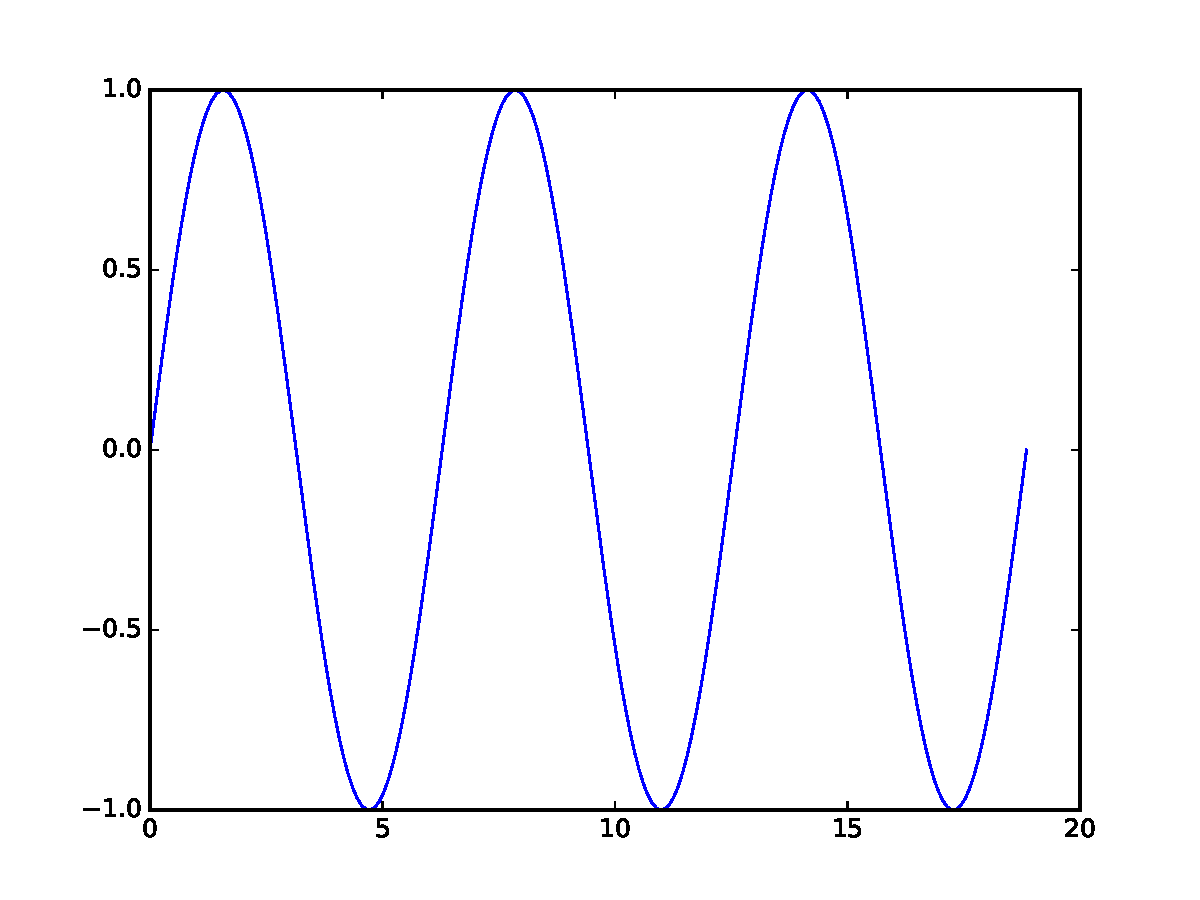
\includegraphics[width= \linewidth]{figures/exemplo_figure3_1.pdf}


\end{document}
